\subsection{Algoritmos para descrição de vídeos}
Estudaremos em detalhes os algoritmos das seguintes seções.


% --------------------------------------------------------------------------------------------------
%
% MEDIDA ORDINAL
%
% --------------------------------------------------------------------------------------------------
\subsubsection{Assinatura de vídeo baseada na medida ordinal}
\label{sec:med_ordinal}

	O algoritmo proposto por \citeauthor{hua2004robust} baseia-se na intensidade dos \textit{pixels} de cada quadro para compor a assinatura. O que se propõe é que, primeiramente, a taxa de amostragem, ou seja, a taxa de quadros por segundo (FPS, do inglês \textit{frames per second}) do vídeo de entrada seja padronizada, para que a assinatura gerada fique mais compacta e seja tolerante a diferentes formatos de compressão, por exemplo. Além disso, o vídeo é convertido para escala de cinza.

Após esse pré-processamento, para cada quadro é realizada a divisão em $M \times N$ blocos, como pode ser observado na Figura \ref{fig:medidaord}, bem como o cálculo da intensidade média para cada um dos blocos. Esses valores são então colocados em ordem crescente e representam cada elemento que compõe a assinatura.

	\begin{figure}[h]
        \centering
        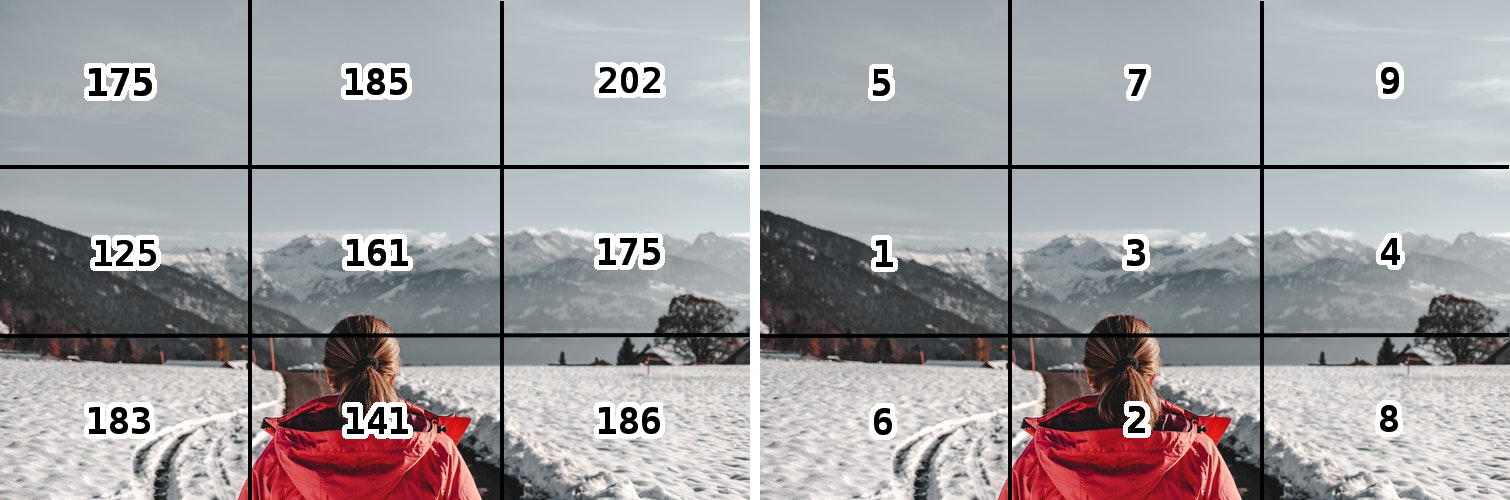
\includegraphics[width=0.8\textwidth]{dados/figuras/mo_final.png}
        \caption{Exemplo com a divisão em blocos, cálculo das intensidades médias e ordem atribuída a cada valor. Referência: \cite{sylvio2015}}
    	\label{fig:medidaord}
    \end{figure}


% --------------------------------------------------------------------------------------------------
%
% GRADIENTE
%
% --------------------------------------------------------------------------------------------------


\subsubsection{Assinatura de vídeo baseada em gradientes}
\label{sec:gradientes}

	Este algoritmo, proposto por \cite{lee2008robust}, utiliza a distribuição dos gradientes para geração de assinaturas. O primeiro passo é definir uma taxa de quadros por segundo (fps) fixa, além da conversão para escala de cinza. Outro procedimento utilizado é o redimensionamento dos quadros, tornando o  método robusto independente da mudança de resolução do vídeo. Em seguida, o gradiente dos \textit{pixels} de cada quadro é calculado da seguinte forma. Encontram-se os gradientes $\mathbb{G}x$ e $\mathbb{G}y$ através da equação \ref{eq:gmatrix}.

\begin{equation}
  \label{eq:gmatrix}
  \begin{bmatrix}
    \mathbb{G}x
    \\ 
    \mathbb{G}y
  \end{bmatrix}= 
  \begin{bmatrix}
    \partial I/\partial x
    \\ 
    \partial I/\partial y
  \end{bmatrix}=
  \begin{bmatrix}
    \mathbb{I}(x+1, y) - \mathbb{I}(x-1,y)
    \\ 
    \mathbb{I}(x, y+1) - \mathbb{I}(x,y-1)
  \end{bmatrix}
\end{equation}
    
	O quadro é então dividido em $M\times N$ blocos, para quais é determinado o valor do centroide dos gradientes, criando assim um vetor com $(M \times N)$ elementos. Para isso, é necessário encontrar a magnitude \textit{$w(x,y)$} e a orientação \textit{$\Theta(x,y)$}, conforme mostra a Equação \ref{eq:mag-or}.
    
\begin{equation}
	\label{eq:mag-or}
    w(x,y) = \sqrt{\mathbb{G}x^{2} + \mathbb{G}y^{2}}
\qquad
\Theta(x,y) = tan^{-1}\left (\frac{\mathbb{G}y}{\mathbb{G}x} \right)
\end{equation}
    
    Em seguida o centroide para cada bloco é obtido a partir do somatório do produto da magnitude e orientação, dividido pela somatória de todas as magnitudes daquele bloco, como pode ser observado na Equação \ref{eq:gradientes}:
    
\begin{equation}
	\label{eq:gradientes}
	[i] = \frac{\sum_{x,y \in b[i]} w(x,y)\Theta (x,y)}{\sum_{x,y \in b[i]} w(x,y)}
\end{equation}
    
% --------------------------------------------------------------------------------------------------
%
% FRAME DIFF
%
% --------------------------------------------------------------------------------------------------

\subsubsection{Assinatura de vídeo baseada na diferença entre quadros}
\label{sec:framediff}

  O algoritmo proposto por \cite{cook2011efficient} utiliza características globais, como luminância e diferença de luminância intra-quadros, para uma assinatura robusta (ao utilizar medidas que refletem a estrutura temporal do conteúdo) e eficiente (ao utilizar medidas simples de serem calculadas e comparadas). Para cada quadro de um vídeo são coletadas as seguintes características: 

  \begin{itemize}
    \item \textit{timestamp}, o tempo do quadro relativo ao início do vídeo
    \item Luminância Total ($Y$), soma da luminância de todos os pixels de um frame
    \item Luminância Máxima ($Y_{max}$), o valor do pixel mais brilhante do quadro
    \item Área do Frame ($A$), largura $\times$ altura do vídeo, útil para normalização
    \item Luminância diferencial ($dY$), a diferença absoluta de luminância pixel a pixel do quadro atual como quadro que estava visível há 100 milisegundos, a diferença resultante é somada (como mostra a equação \ref{eq:framediff}). 
  \end{itemize}

\begin{equation}
	\label{eq:framediff}
	dY = \sum_{x,y \in  \mathbb{I,J}} |\mathbb{I}(x,y) - \mathbb{J}(x,y)|
\end{equation} 

  Após a obtenção das características primárias, estas passam por um processo de refinamento no qual os vetores $Y$ e $dY$ são passados por filtros passa-baixa (figura ~\ref{fig:framediff-passa-baixa}). Além disso, duas outras características são derivadas das características principais e visam medir o quão imóvel uma sequência de frames é. Para isso, são definidas as medidas "Quietude" (equação \ref{eq:framediff-credits}) e "Créditos" (equação \ref{eq:framediff-stillness}).

  \begin{equation}
    \label{eq:framediff-stillness}
    Quietude = 100 \times \left(\sqrt{\frac{\ln\frac{dY}{A}}{\ln256}}\right) \\
  \end{equation}

  \begin{equation}
    \label{eq:framediff-credits}
    Creditos = 100 \times \frac{\frac{Y_{max}}{256} + \left( 1 - \left( \frac{\ln\frac{Y}{A}}{\ln256} \right)^2\right)}{2}
  \end{equation}


\begin{figure}[h]
  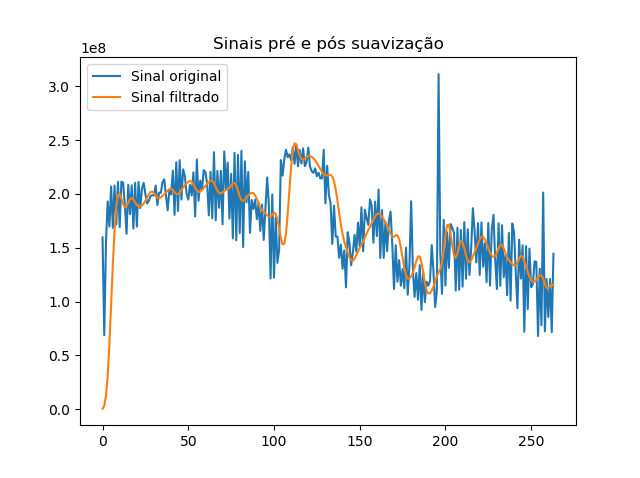
\includegraphics[width=0.7\textwidth]{dados/figuras/filtro_passa_baixa}
  \caption{Linha azul mostra os valores originais do vetor $dY$ e a linha alaranjada mostra os valores pós filtro passa-baixa}
  \label{fig:framediff-passa-baixa}
\end{figure}


A figura \ref{fig:framediff-comparacao} mostra a característica $dY$ plotada para um vídeo original e sua versão distorcida com efeitos de desfoque (\textit{blur}) e adição de legenda, além de mostrar os valores de $dY$ para outro vídeo não relacionado.

\begin{figure}[h]
  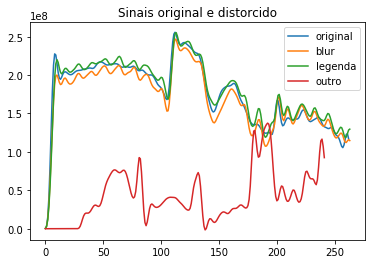
\includegraphics[width=0.7\textwidth]{dados/figuras/dy}
  \caption{Comparação entre os vetores de característica $dY$ gerados para um vídeo, uma cópia com o efeito de desfoque, uma cópia com uma legenda inserida, e um outro vídeo qualquer}
  \label{fig:framediff-comparacao}
\end{figure}


Para realizar a comparação entre duas assinaturas, \citeauthor{cook2011efficient} propõe o uso da distância de Manhattan normalizada, como descrito na fórmula \ref{eq:dist-manhattan}. Além disso, é proposto o uso de uma combinação das características $Y$ e $dY$ na comparação, pois separadas elas obteram $0.579\%$ e $0.157\%$ de falsos positivos, respectivamente, enquanto que a combinação das duas características obteve apenas $0.018\%$. 

\begin{equation}
  Distancia(a,b) = \frac{\sum_i|a_i - b_i|}{|a|}
  \label{eq:dist-manhattan}
\end{equation}

%% --------------
%% TODO: explicar comparação
%% --------------

%   Dados dois quadros $\mathbb{I}$ e $\mathbb{J}$, a assinatura temporal desenvolvida por \cite{cook2011efficient} utiliza dois componentes principais para sua construção. O primeiro é a luminância total $Y$, ou seja, a soma dos \textit{pixels} do \textit{frame}, representando o brilho total da imagem. O outro parâmetro é $dY$, ou diferencial de luminância, sendo a diferença do quadro atual com o quadro anterior. $dY$ é uma métrica para saber o quanto a luminância varia com a mudança dos quadros no vídeo.  Essa variação pode acontecer, segundo o autor, a partir do movimento da câmera, corte entre cenas e objetos e pessoas que entram ou saem de cena. 
    
%    O  valor de $dY$ pode ser obtido através da Equação \ref{eq:framediff} \cite{sylvio2015}: 

% Portanto cada \textit{frame} será representando por uma tupla $(Y, dY)$.
    
% --------------------------------------------------------------------------------------------------
%
% WAVELETS
%
% --------------------------------------------------------------------------------------------------

\subsubsection{Assinatura de vídeo baseada em wavelets}

Esta abordagem foi escolhida por ter sido projetada especialmente para ser robusta a uma variedade de ataques fotométricos e de pós-produção, como modificações em contraste, brilho, contaminação por ruído e desfoque, inserção de logos, bordas e mudança de formato do quadro. Para se tornar ainda mais robustas a estes ataques, \citeauthor{Dutta2013} também descreve um fluxo de pré-processamento.

Após a etapa de pré-processamento, para ser utilizado como entrada para este algoritmo, os vídeos devem ser transformados para escala de cinza e ter suas intensidades normalizadas para o intervalo $[0,1]$. A assinatura proposta por \citeauthor{Dutta2013} é composta de uma parte baseada na transformada de Haar e em  outra baseda na distribuição espacial de gradientes.

\subsection{Obtenção da assinatura}

\begin{enumerate}
\item Seja $I$ a imagem obtida após conversão para escala de cinza e normalização
% \item $F_i$ <- $F$
\item Para i de 1 até $n$, onde $n$ é o número de iterações da transformada de Haar
  \begin{enumerate}
    \item Aplicar a transformada de Haar sobre $I$ para obter um vetor com ($LL, LH, HL, HH$)
    \item Computar energia de $LH$, $HL$, $HH$ \footnote{$  \frac{1}{MN}\sum_{x=1}^M \sum_{y=1}^N |\mathbb{I}(x,y)|$}
  \end{enumerate}
\item Computar a energia da subimagem $I$, do último valor de $LL$ e concatenar estes valores em um vetor,
\item Concatenar os valores de energia obtidos nos passos anteriores para obter o descritor
\end{enumerate}

\begin{figure}[h]
  \centering
  \begin{tabular}{ccc}
    \centering
    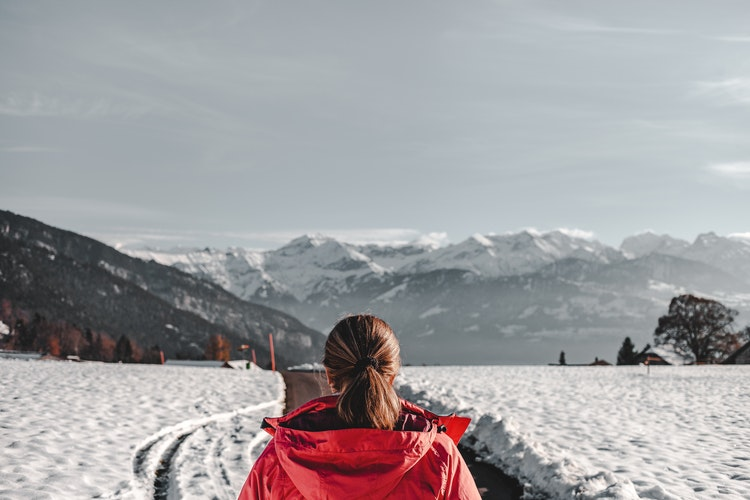
\includegraphics[width=0.45\textwidth]{dados/figuras/original} & 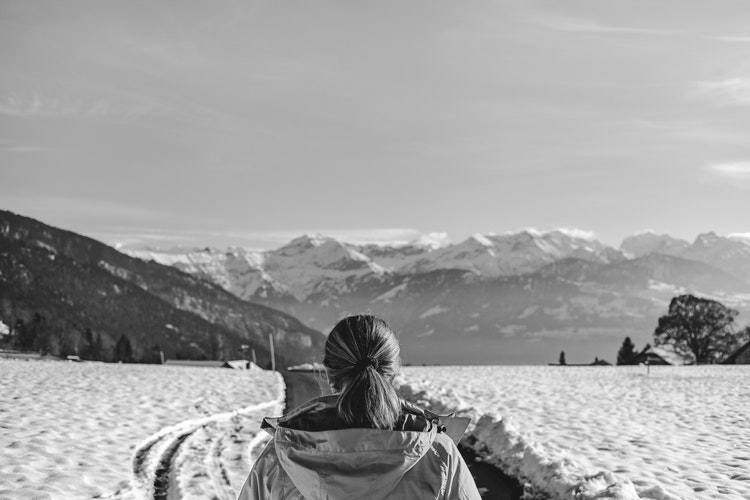
\includegraphics[width=0.45\textwidth]{dados/figuras/original_bw} \\ 
     a. Quadro original & b. Quadro em escala de cinza \\
    \multicolumn{2}{c}{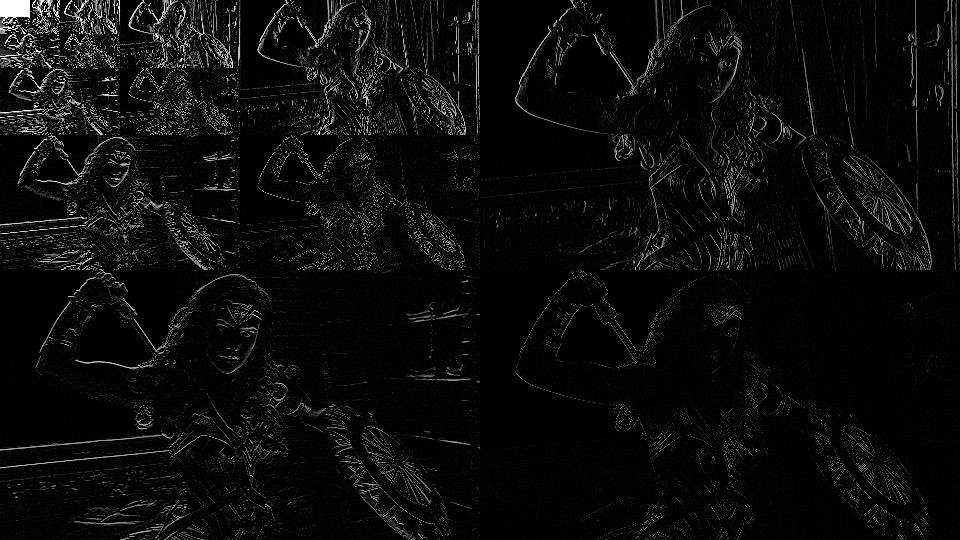
\includegraphics[width=0.94\textwidth]{dados/figuras/ww_haar_}} \\
    \multicolumn{2}{c}{c. Após transformada de Haar}
  \end{tabular}
  \caption{Sequência de transformações feitas pelo algoritmo}
%   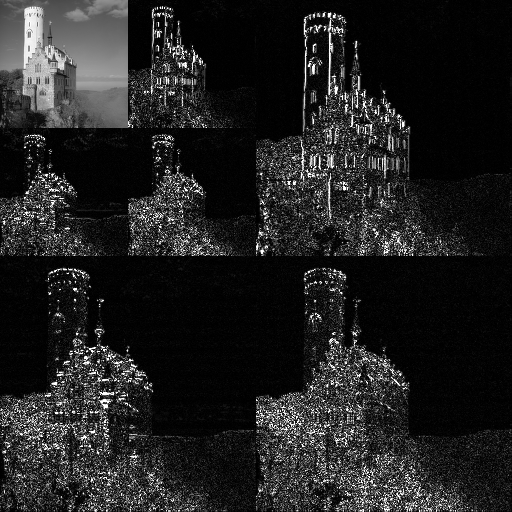
\includegraphics[width=0.8\textwidth]{dados/figuras/haar.png}
%   \caption{Resultado da Transformada de Haar. Os cantos superior direito, inferior esquerdo e inferior direito são, respectivamente, a derivada na horizontal(LH),derivada na vertical(HL) e derivada na diagonal(HH). O canto superior esquerdo é subdividido $N$ vezes em LH,HL e HH até o último nível em que não há mais divisão e que se chama LL}
  \label{figure:haar}
\end{figure}

\subsubsection{Assinatura baseada em distribuição espacial de gradientes}

\begin{enumerate}
\item Dado um quadro $I$ já pré-processado, aplicar a transformada de Haar com um nível e obter um vetor com $LL,LH,HL,HH$
\item Computar o gradiente de $LL$\footnote{A imagem LL é usada pois contém menos ruído que a imagem original graças à transformada de Haar}
\item Dividir a imagem de gradiente em $N_p$ partições com o mesmo tamanho
\item Para cada partição, computar um histograma de gradiente
\item Concatenar os histogramas  para obter o descritor
\end{enumerate}

% --------------------------------------------------------------------------------------------------
%
% SCENE FRAME
%
% --------------------------------------------------------------------------------------------------

\subsubsection{Assinatura baseada em quadros de cena}

  Outra abordagem, proposta por \citeauthor{mao2015sceneframe}, é baseada na assinatura de quadros de cena. De acordo com os autores, os quadros de cena podem ser \textit{intraframes}, ou seja, quadros que iniciam tomadas, quanto \textit{interframes}, contanto que sigam as características descritas em \ref{sec:quadrocena}.
    
    O algoritmo fundamenta-se na ideia de que as chances de existirem cinco quadros de cena seguidos é extremamente baixa, por isso são selecionados apenas os cinco primeiros quadros de cena de um vídeo. A forma como estes são determinados é descrita na Seção \ref{subsec:fptsceneframe}.

\subsection{A extração de assinatura}
\label{subsec:fptsceneframe}

% \begin{algorithm}
	\caption{HUGO \cite{hugo}}
	\label{alg:hugo}
	\KwIn{Todos os PIXELS da imagem de cobertura X}
	\KwOut{A estego imagem Y}

	\For { $(i, j)$ in $PIXELS$ } {

        \tcp{Calcula o impacto da codificação de +1}

		\algstat{stego\_plus \gets X.copy()}

		\algstat{stego\_plus[i][j]++}

		\algstat{embed\_impact\_plus[i][j] \gets D(X, stego\_plus)}

        \tcp{Calcula o impacto da codificação de -1}

		\algstat{stego\_minus \gets X.copy()}

		\algstat{stego\_minus[i][j]--}

		\algstat{embed\_impact\_minus[i][j] \gets D(X, stego\_minus)}
	}

	\tcp{Mínimo, elemento a elemento}

	\algstat{embed\_impact\_min \gets min(embed\_impact\_plus, embed\_impact\_minus)}

	\tcp{\textit{Syndrome Trellis-Code}}

	$\mathrm{pixels\_to\_change} \gets \mathrm{minimize\_embed\_impact}(LSB(X), \mathrm{embed\_impact\_min, message})$

	\algstat{Y \gets X}

	\eIf{ \algstat{model\_correction\_step\_enabled} } {
		\For { $(i, j)$ in $pixels\_to\_change$ } {
			\algstat{correction\_plus \gets Y}

			\algstat{correction\_plus[i][j]++}

			\algstat{dp \gets D(X, correction\_plus)}

			\algstat{correction\_minus \gets Y}

			\algstat{correction\_minus[i][j]--}

			\algstat{dm \gets D(X, correction\_minus)}

			\eIf{ $dp < dm$ }{
				$Y[i][j]++$
			}{
				$Y[i][j]--$
			}
		}
	}{
		\For { $(i, j)$ in $pixels\_to\_change$ } {
			\eIf{ $embed\_impact\_plus[i][j] < embed\_impact\_minus[i][j]$ }{
				$Y[i][j]++$
			}{
				$Y[i][j]--$
			}
		}
	}
	
\end{algorithm}


A obtenção da assinatura, para \citeauthor{mao2015sceneframe}, é realizada para todos os quadros, para então serem comparadas e selecionadas. Como pode ser observado no Diagrama \ref{dig:sceneframe}, os quadros passam por um pre-processamento, onde o componente de luminância é obtido. O quadro então é recortando, mantendo-se apenas sua região central e, por fim, redimensionado para o tamanho definido de $3/4$QCIF, ou seja, $(108\times132)$.

% Após o processamento inicial, o quadro é então dividido em $144$ pedaços menores, de tamanho $(9\times11)$, cuja média de intensidade irá compor parte da assinatura deste quadro. Além dos $144$ valores, o descritor é composto também por $576$ elementos diferenciais, totalizando $720$ valores. Para obter esses elementos, cada fragmento é dividido em oito elementos menores, como mostra a Figura \ref{fig:divsceneframe}, e então é realizada a subtração de $a - b$, $c - d$, $e - f$ e $g - h$.

\begin{figure}[h]
  \centering
    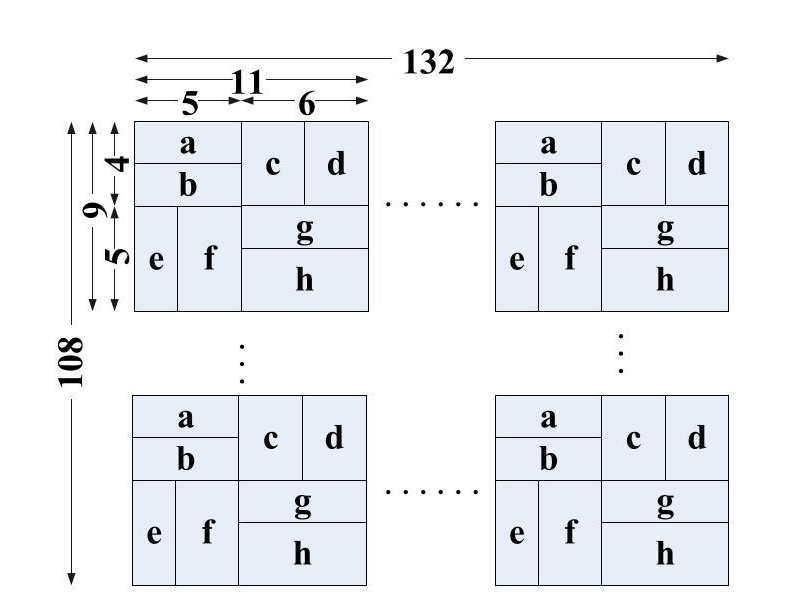
\includegraphics[width=\textwidth]{dados/figuras/sf_division.png}
    \caption{Divisão da imagem para cálculo dos elementos diferenciais. Referência: \citeauthor{mao2015sceneframe}}
    \label{fig:divsceneframe}
\end{figure}

\subsection{Diminuição do espaço de memória utilizado}

O artigo também propõe uma alternativa para diminuir o espaço de memória utilizado para armazenar as assinaturas, visto que o banco de dados dos vídeos pode ser grande. Para isso, é proposta uma técnica chamada qualificação quaternária, na qual os valores são classificados de acordo com um \textit{threshold}.


% --------------------------------------------------------------------------------------------------
%
% RBP
%
% --------------------------------------------------------------------------------------------------